%\documentclass[12pt]{article}
\documentclass[11pt]{revtex4}
\usepackage[dvipdf]{graphicx}
\usepackage{color}
\usepackage{multirow}
\usepackage{subfigure}  % For subfloats
\usepackage{epsfig}
\usepackage{wrapfig}
\usepackage{rotating}
\usepackage{graphicx}
\usepackage{amsmath}
%
\newcommand{\JLAB}{Thomas Jefferson National Accelerator Facility, Newport News, Virginia 23606}
\newcommand{\JP}{J/$\psi~$}
%
\begin{document}
\title{ Artificial Intelegence for CLAS12 Tracking}


\author{G. Gavalian}
\affiliation{Thomas Jefferson National Accelerator Facility, Newport News, VA 23606}
%

\date{\today}

\begin{abstract}
%{\footnotesize {\bf Abstract}   }
{{\bf Abstract.}
This document describes AI projects that we think can help CLAS12 workflow.
}
\end{abstract}
\maketitle
%\end{document}
%\tableofcontents
%\clearpage

\vspace{1in}

\section{Introduction}

In this document we provide possible areas where AI can aid CLAS12 software
to improve either performance or reliability.

\section{Tracking}

In CLAS12 charged particle tracks are measured using Drift Chambers inside of
toroidal magnetic field. Drift Chambers consist of 6 super-layers, each super-layer
 consisting of 6 layers of wires, each layer containing 112 wires, running perpendicular
 to particle direction.

In data reconstruction process segments measured by each super layer are combined
to form a track candidate. Each track candidate is fitted to determine initial
track parameters. Then track candidates are fitted using Kalman-Filter.
During high luminosity running there are many track candidates formed from
combinations of segments from size super-layers. Fitting all track candidates
is computationally intensive and 94\% if time in detector reconstruction program
is spend on tracking.

Modern advances in Artificial Intelligence inspired us to develop neural network
to evaluate track candidates quality based on prior training on reconstructed data.
This work was done in collaboration with CRTC computing center at Old Dominion University.

\begin{figure}[htb]
\begin{center}
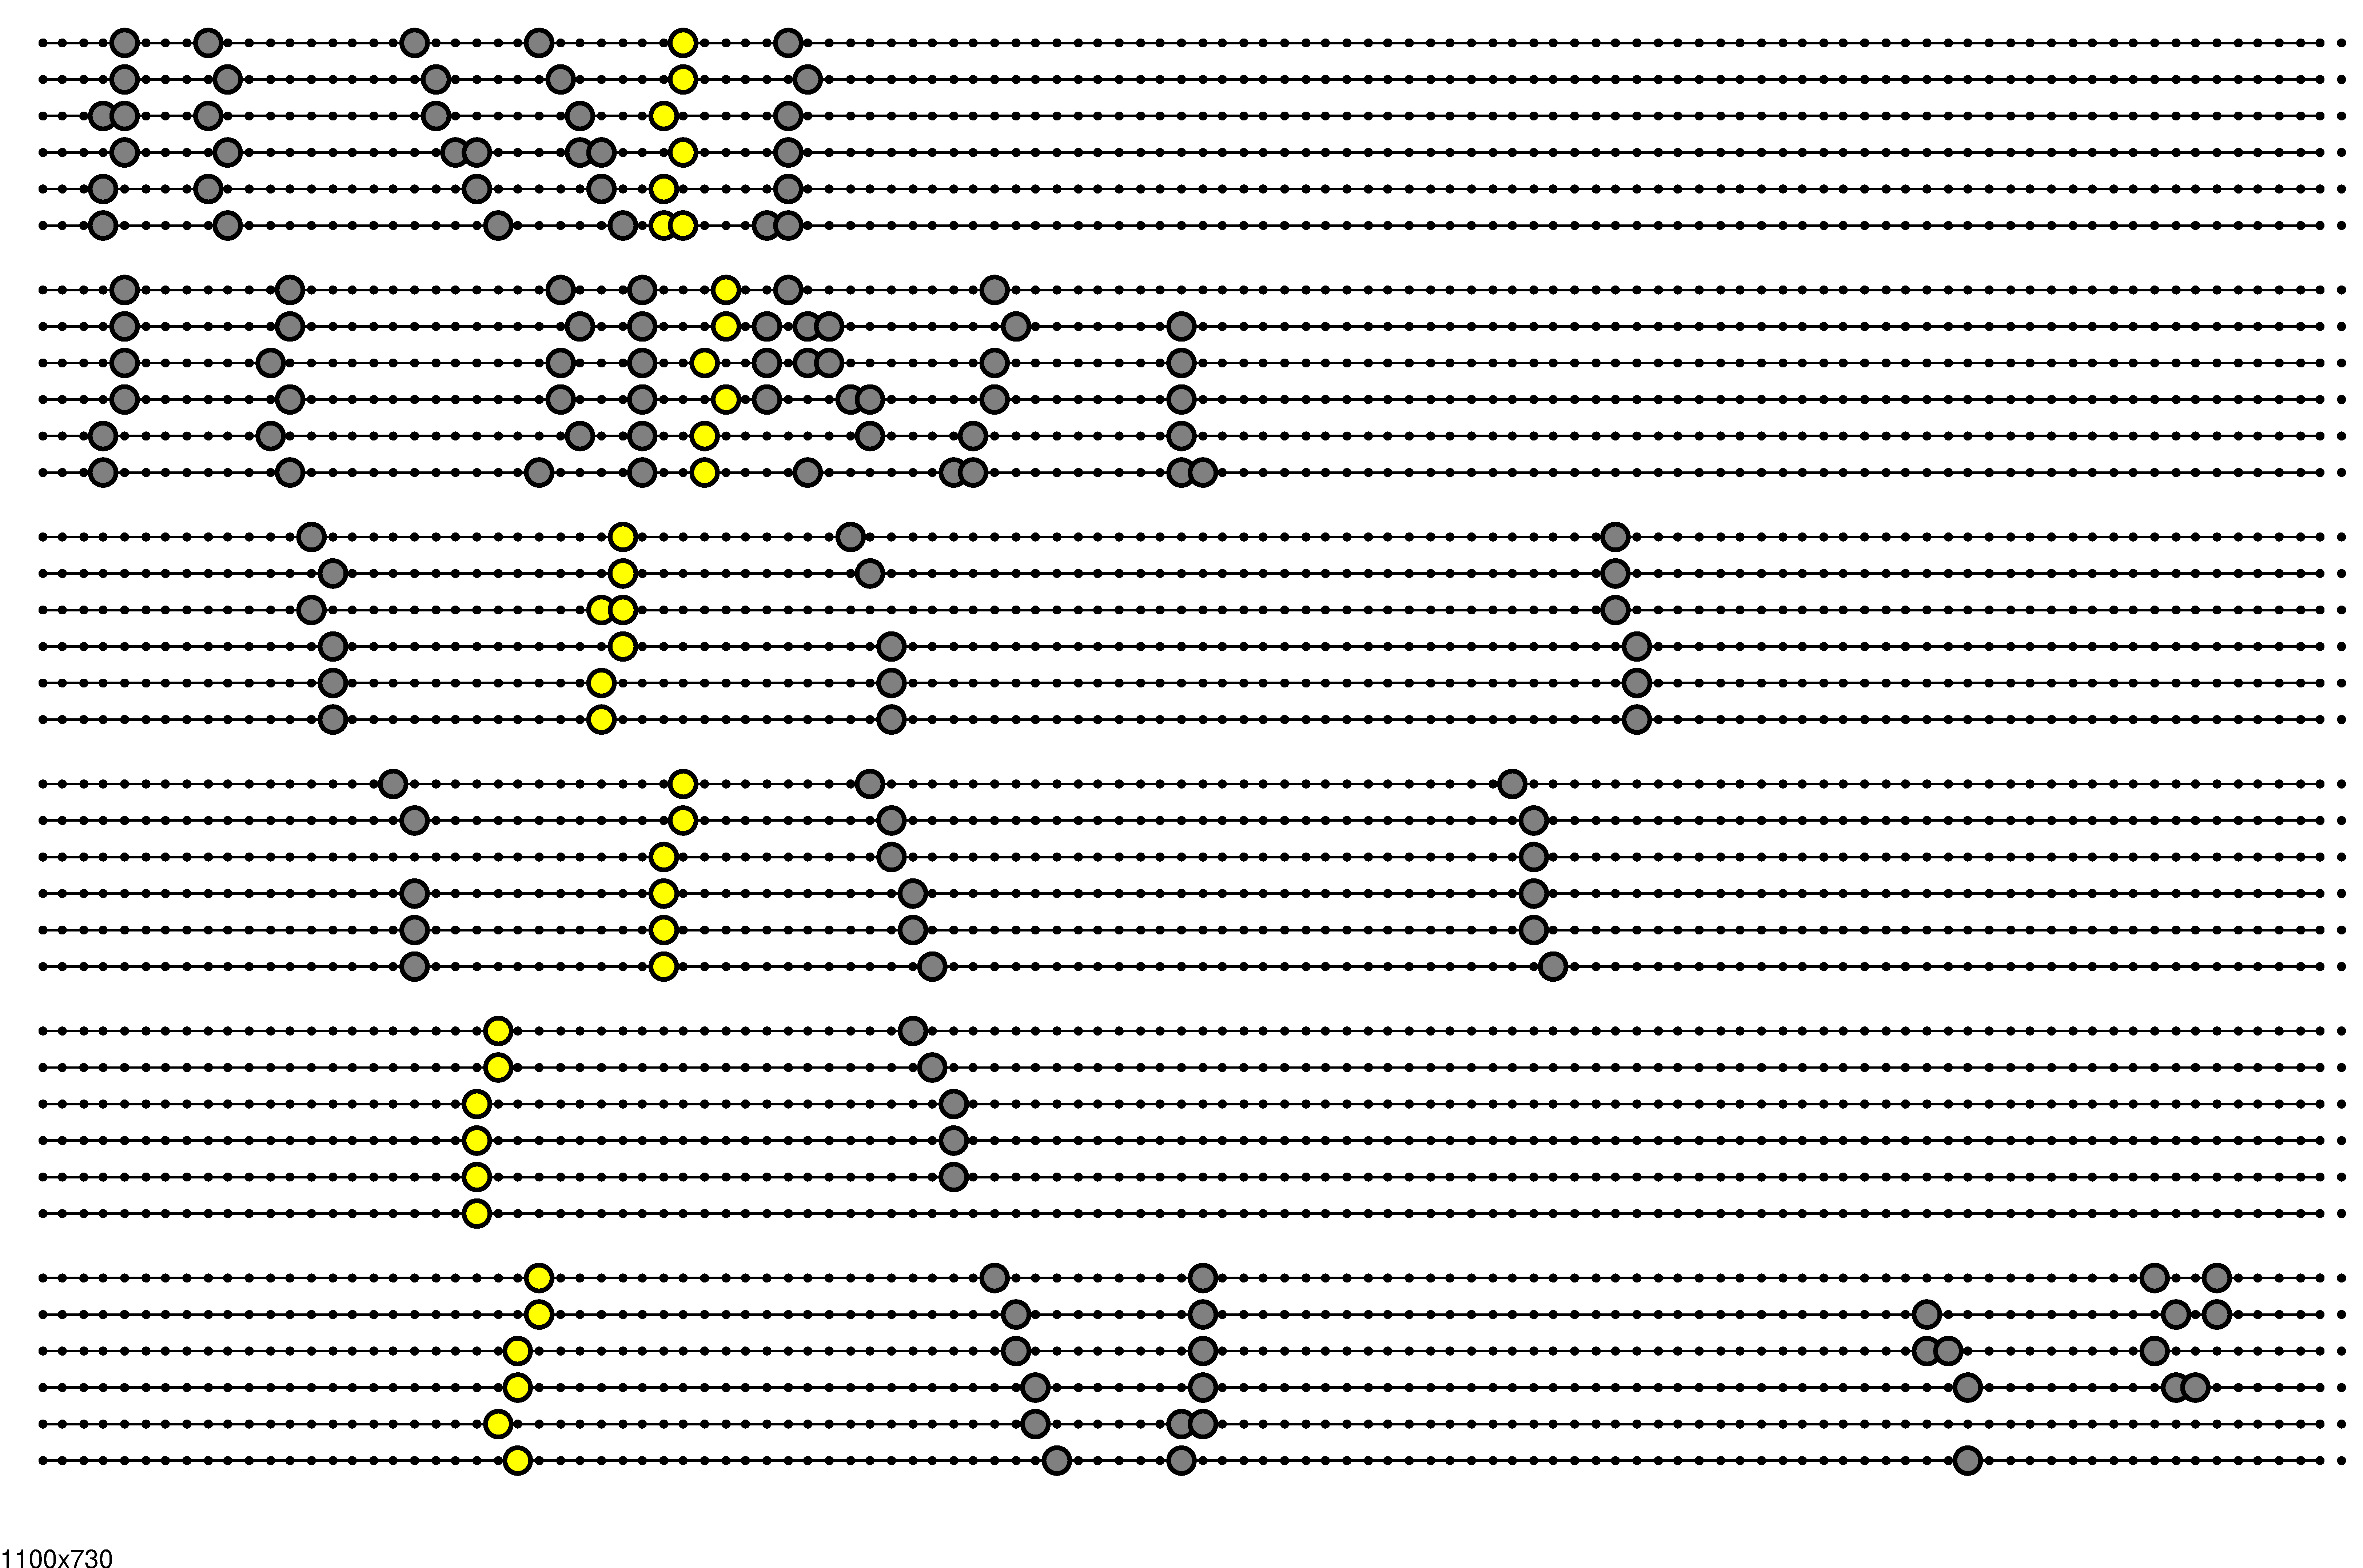
\includegraphics[width=2.5in]{dc_image_set_1_positive}
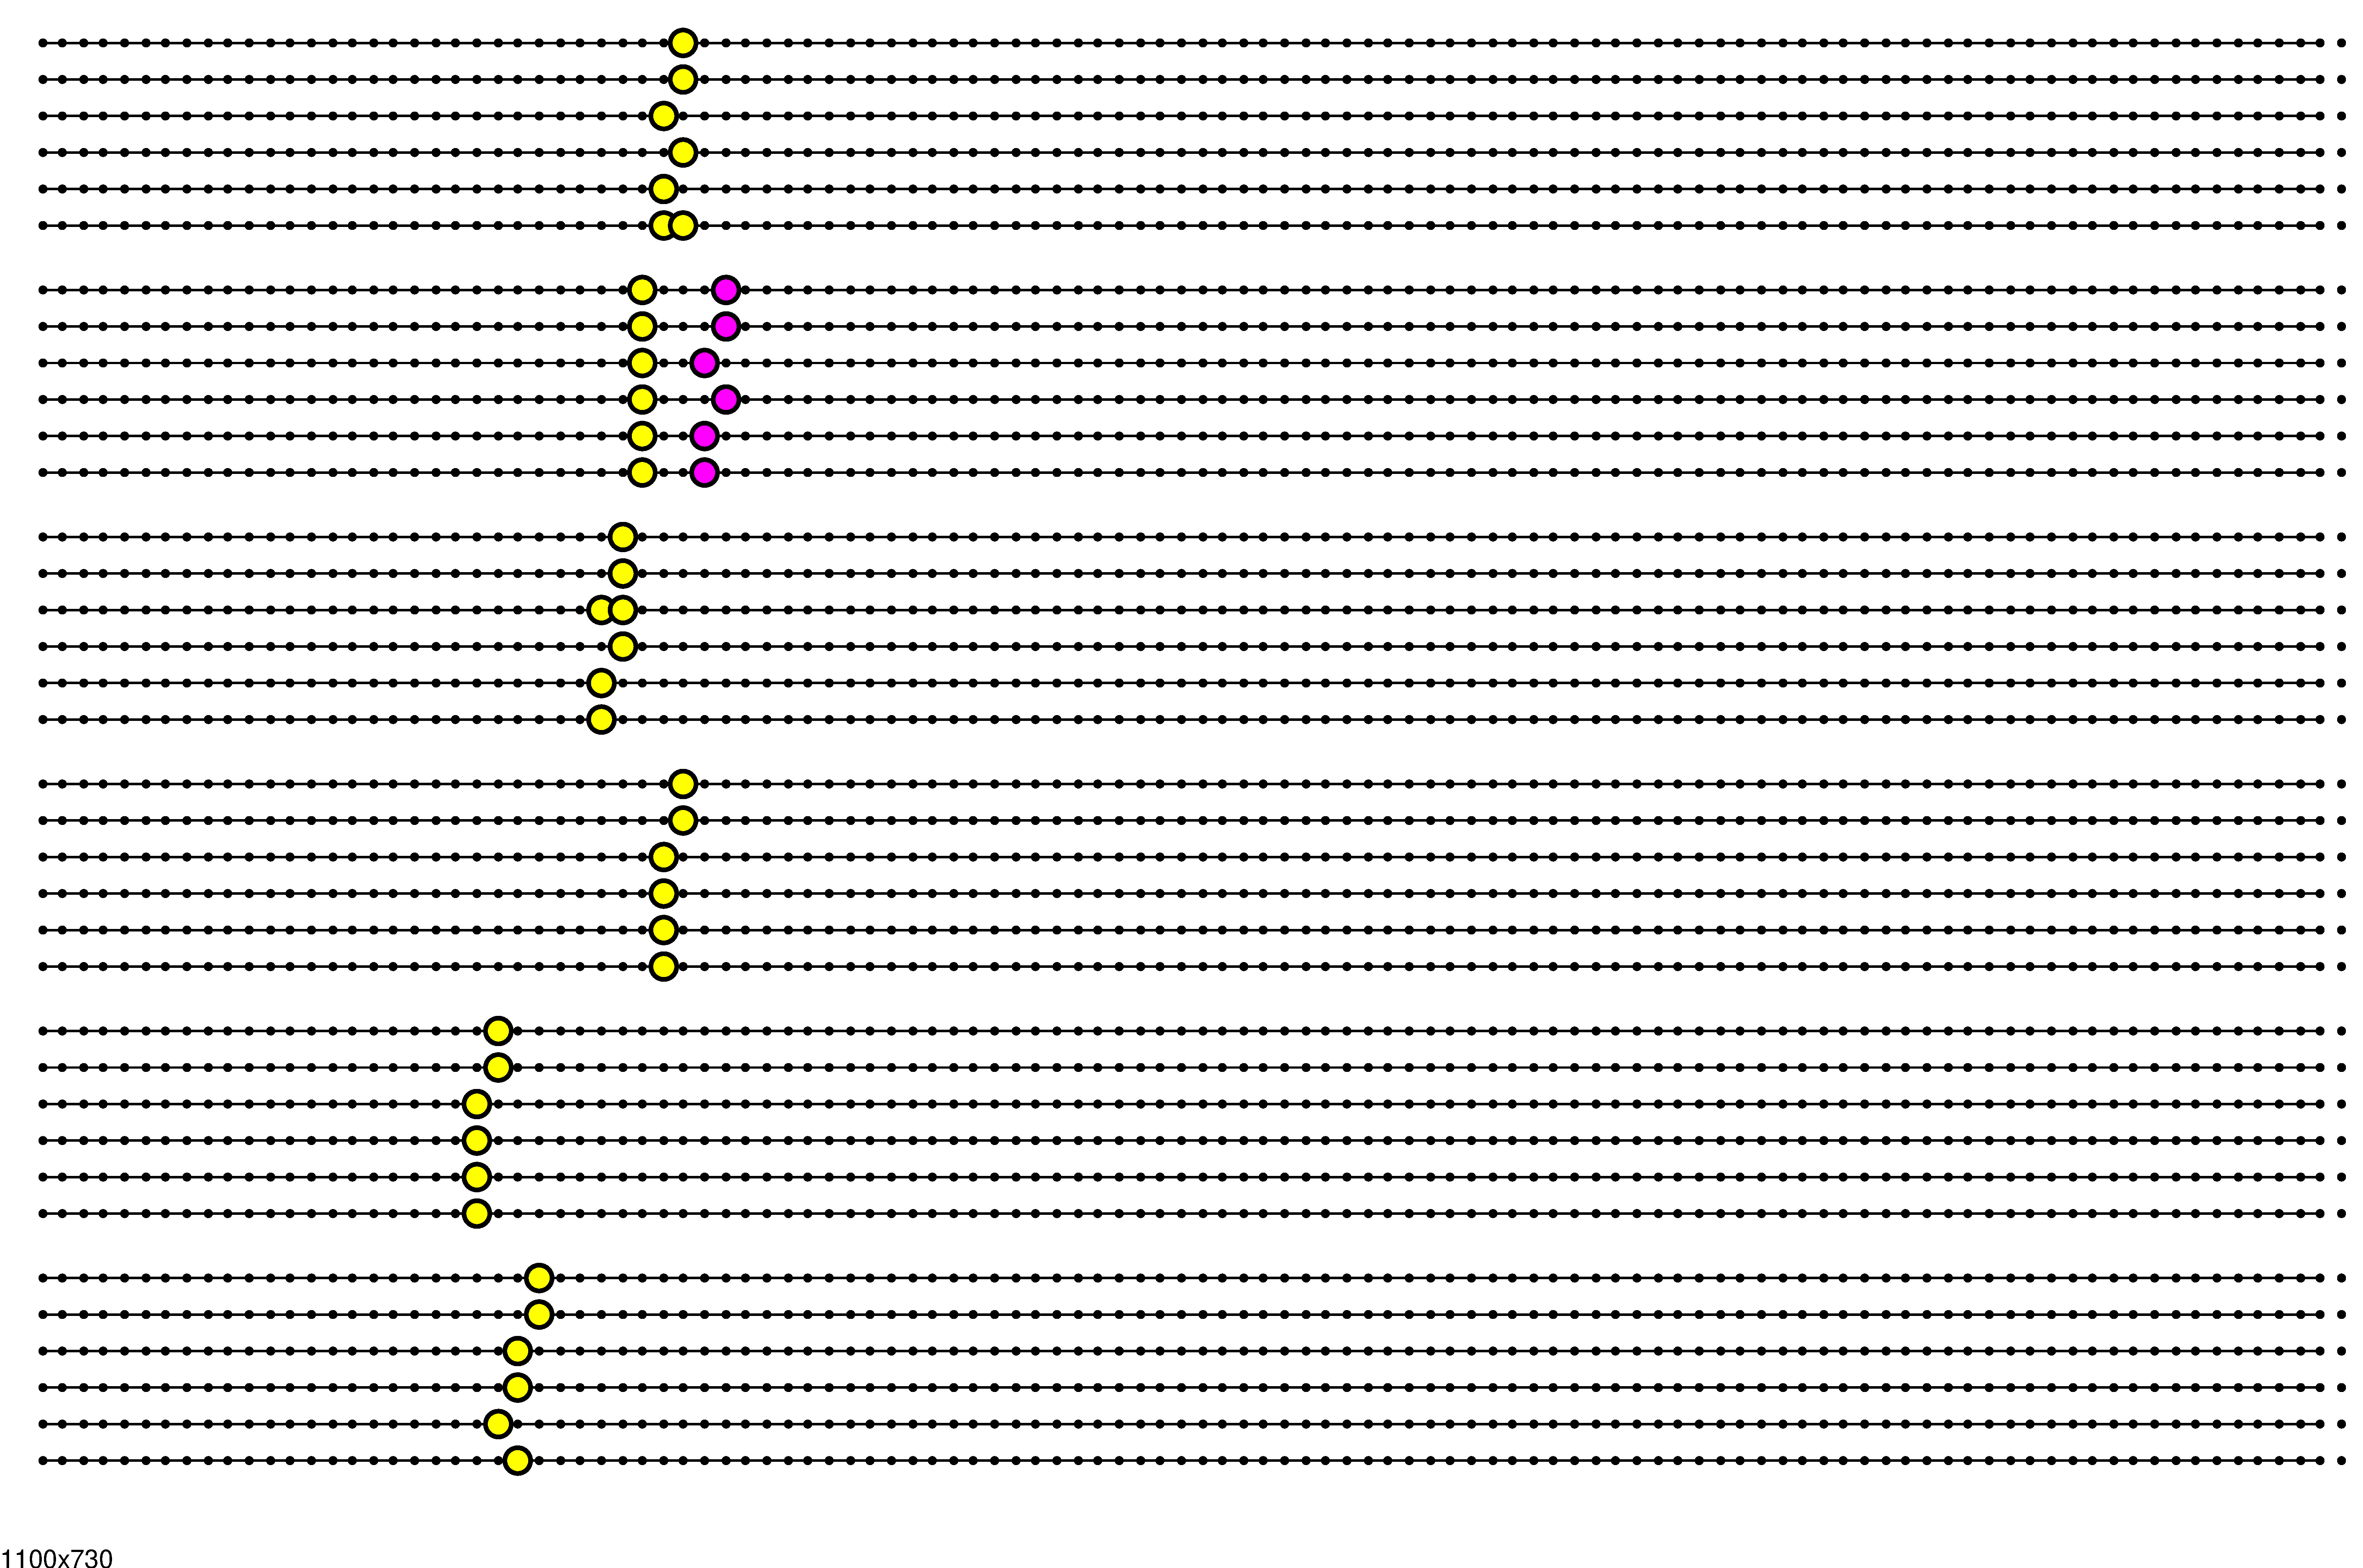
\includegraphics[width=2.5in]{dc_image_set_1_negative}
\caption{This is a figure.}
\end{center}
\end{figure}

Three different network types were investigated to assess accuracy of track classifications,
namely Convolutional Neural Network (CNN), Extreamly Randomized Tree (ERT) and
Multy-Layer Perceptron (MLP). The results from each network can be seen in
Table ~\ref{tbl:RESULTS}.

\begin{table}[!h]
\begin{tabular}{|l|c|c|c|}
\hline
Network & Training Accuracy & Validation Accuracy & Inference Time \\
\hline
\hline
Convolutional Neural Network & 94.26\% & 90.15\% & 1.2 ms \\
Extreamly Randomized Tree & 99.99\% & 91.90\% & 5  $\mu s$ \\
Multilayer Perceptron & 98.41\% & 99.2\% & 4  $\mu s$ \\
\hline
\end{tabular}
\caption{Performance of Neural Networks investigated for track classification.}
\label{tbl:RESULTS}
\end{table}

As a result of tests we decided to use MLP network due to higher accuracy of classification
and faster inference time ($\approx 4 ~\mu s$). We implemented AI predictions into our
reconstruction workflow, where only track candidates found by neural network were fitted
by tracking algorithm using Kalman-Filter. Our preliminary results show that $\approx 99\%$
of tracks are reconstructed and tracking speed has improved by factor of 6, due to significant
decrease of combinations of segment considered for track candidates.

\end{document}
